\documentclass{article}
\usepackage[utf8]{inputenc}
\usepackage[english]{babel}
\usepackage [autostyle, english = american]{csquotes}
\MakeOuterQuote{"}
\usepackage{graphicx}
\usepackage{enumerate}
\usepackage{float}
\graphicspath{ {} }
\usepackage{mathtools}
\usepackage{amsmath, amsthm, amssymb, amsfonts}
\usepackage{caption}
\usepackage{bm}
\usepackage{fancyhdr}
\pagestyle{fancy}
\fancyhf{}
\rhead{Ty Darnell}
\lhead{Qaqish Review Session 1}

% For derivatives
\newcommand{\deriv}[1]{\frac{\mathrm{d}}{\mathrm{d}x} (#1)}

% For partial derivatives
\newcommand{\pderiv}[2]{\frac{\partial #1}{\partial #2}}

% Integral dx
\newcommand{\dx}{\mathrm{d}x}
\newcommand{\cd}{\overset{d}{\to}}
\newcommand{\cp}{\overset{p}{\to}}
\newcommand{\B}{\beta}
\newcommand{\e}{\epsilon}
\newcommand{\limn}{\lim_{n\to \infty}}
\newcommand{\lm}{\lambda}
\newcommand{\sg}{\sigma}
\newcommand{\hb}{\hat{\beta}}
\newcommand{\sumn}{\sum_{i=1}^{n}}
\newcommand{\hth}{\hat{\theta}}
\newcommand{\lra}{\Leftrightarrow}
\newcommand{\prodn}{\prod_{i=1}^{n}}
\newcommand{\dll}[1]{\dfrac{\partial\ell}{\partial{#1}}}
\newcommand{\mle}{\hat{\theta}_{MLE}}
\newcommand{\mm}{\hat{\theta}_{MM}}
\newcommand{\sumx}{\sum_{i=1}^{n}x_i}
\newcommand{\ta}{\theta}
\newcommand{\qe}{ \ ?\ }
\newcommand{\dt}{\pderiv{}{\ta}}
\newcommand{\lt}[1]{\log(f(#1|\ta))}
\newcommand{\lx}{\lambda(x)}
\newcommand{\samp}{X_1,\dots,X_n \sim}
\newcommand{\te}{\theta_1}
\newcommand{\xm}{x_{(1)}}
\newcommand{\sn}{(\sg^2)}
\newcommand{\pow}{\B(\ta)}
\newcommand{\hyp}[2]{H_0: #1 \text{ vs } H_1: #2}
\newcommand{\pois}[2]{\dfrac{e^{-#1}{#1}^{#2}}{{#2}!}}
\newcommand{\mlr}{\dfrac{f(x|\ta_2)}{f(x|\ta_1)}}
\newcommand{\al}{\alpha}
\newcommand{\bx}{\bar{x}}
\newcommand{\ra}{\Rightarrow}
\allowdisplaybreaks
\begin{document}
\begin{flushleft}
Old quals link: \underline{bios.unc.edu/distrib/exam/ms}
\section*{General Advice From Qaqish}
\begin{itemize}
\item 3 problems 6 hours
\item Read question for about 30 minutes, important that you fully understand question before you start working. Read and reread
\item Don't jump to quick conclusions, find a shorter way to solve problem. Don't make kneejerk assumptions
\item Conditional Distribution- use double expectation to find $E(X), Var(X), Cov$
\item Just because you can't do part a does not mean you can't do parts b and c, etc
\item For biased/unbiased estimator questions answer yes/no, don't automatically find $E(X)$\\
ex: $\bar{X^2}$ est of $\mu^2 \quad \mu=E(X)$\\
Jensen's inequality: if $g(x)$ convex then $E[g(x)]>g(E[X])$\\
$g(x)=X^2 \ra$ convex\\
$E(X^2)>(E(X))^2=\mu^2$ Thus biased
\end{itemize}

\section*{2017 Quals Problem 1}
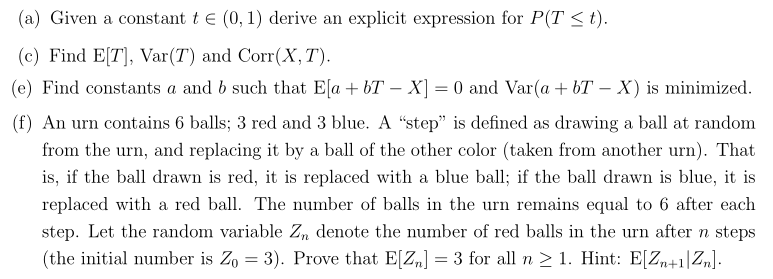
\includegraphics[scale=.65]{images/qual1.png}	
\begin{enumerate}[(a)]
\pagebreak	
	\item 
\begin{multline*}\\
f_Y(y)=e^{-y} \quad y>0\\
x\in (0,1) \quad y \in (0,\infty)\\
T=X+Y\\
\text{given } t\in (0,1) \\
P(X+Y\leq t)\\
\{X+Y\leq t \} \text{ (event)}\\
=\{y\leq t-x \} \text{ (plot)}\\
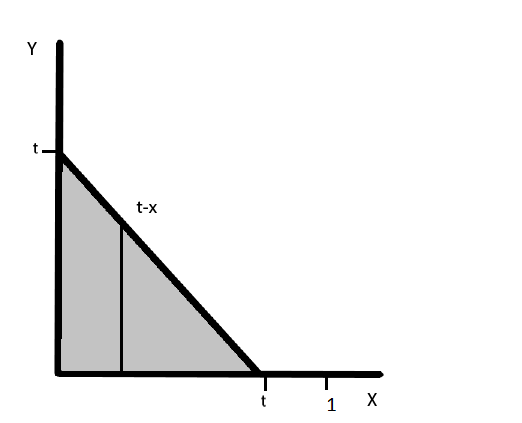
\includegraphics[scale=.5]{images/2017plot1.png}\\
\text{integrate x from 0 to t}\\
\text{for each x, integrate y from 0 to t-x}\\
\int_{x=0}^{x=t}\int_{y=0}^{y=t-x}f_{X,Y}(x,y) \ dy \ dx \qquad f_{X,Y}(x,y)=e^{-y}\\
\int_{0}^{t}\int_{0}^{t-x}e^{-y}\ dy \ dx\\
\ra \int_{0}^{t}1-e^{-(t-x)} \dx \ra t-1+e^{-t}\\
P(T\leq t)= t-1+e^{-t}\\
\end{multline*}

\stepcounter{enumi}
	\item 
\begin{multline*}\\
\text{Find } E(T) \quad Var(T) \quad Corr(T)\\
E(T)=E(X)+E(Y)=1/2+1=3/2\\
Var(T)=Var(X)+Var(Y)+Cov(X,Y)\\
=1/12+1+0 \quad (X\perp Y)\\
Var(T)=13/12\\
T=X+Y\\
Cov(X,T)=Cov(X,X+Y)\ra Cov(X,X)+Cov(X,Y)\\
=Var(X)+0=1/12\\
Cov(X,T)=1/12\\
Corr(X,T)=\dfrac{Cov(X,T)}{\sqrt{Var(X)Var(T)}}=\dfrac{1/12}{\sqrt{(1/12) (13/12)}}=\dfrac{1}{\sqrt{13}}\\
\end{multline*}

\stepcounter{enumi}

\item 
\begin{multline*}\\
\text{find a and b s.t. } E(a+bT-X)=0 \text{ and } Var(a+bT-X) \text{ is minimized}\\
\text{Since } E(T)=1.5 \quad E(X)=.5 \text{ we have:}\\
E(a+bT-X)=a+b(1.5)-.5\\
b=\dfrac{.5-a}{1.5}\\
Var(a+bT-X)=0+Var(bT)+Var(X)-2Cov(bt,X)\\
=b^2(13/12)+1/12-2bCov(T,X)\\
=b^2(13/12)+1/12-2b/12\ra (1/12)(13b^2-2b+1) \text{ (convex)}\\
\dfrac{d}{d b}=(1/12)(26b-2)=0 \text{ (minimizing)}\\ 
\ra b=13\\
\text{Plugging back into } b=\dfrac{.5-a}{1.5} \text{ we get:}\\ 
13*1.5=.5-a\\
\ra a=-19\\
\text{Thus } a=-19, b=13\\
\end{multline*}

\item 
\begin{multline*}\\
\begin{array}{c|c}
Red & Blue\\
\hline
3 & 3\\
Z_n & 6-Z_n
\end{array}\\
P(\text{Red Ball}|Z_n \text{ currently})=Z_n/6\\
P(\text{Blue}|Z_n)=1-Z_n/6\\
\begin{array}{c|c|c}
\text{Draw} & \text{Red} & \text{Blue}\\
\hline
Red & Z_n-1&6-Z_n+1\\
Blue &Z_n+1&6-Z_n-1\\
\end{array}\\
P(Z_{n+1}=Z_n-1|Z_n)=Z_n/6\\
P(Z_{n+1}=Z_n+1|Z_n)=1-Z_n/6\\
E(Z_{n+1}|Z_n)=(Z_n-1)Z_n/6+(Z_n+1)(1-Z_n/6)\\
=-Z_n/6+Z_n+1-Z_n/6\\
E(Z_n+1|Z_n)=1+(2/3)Z_n\\
E(Z_1|Z_0=3)=3\\
E(Z_2|Z_1)=1+(2/3)Z_1\\
E(E(Z_{n+1}|Z_n))=E(Z_n+1)\\
E(Z_{n+1})=1+(2/3)E(Z_n)\\
\text{In the form of: } a=1+(2/3)a \ra (1/3)a=1\ra a=3\\
\end{multline*}

\end{enumerate}


\end{flushleft}
\end{document}
